%*******************************************************************************
%*********************************** First Chapter *****************************
%*******************************************************************************

\chapter{Estado del Arte}  %Title of the Second Chapter

\ifpdf
    \graphicspath{{Chapter2/Figs/Raster/}{Chapter2/Figs/PDF/}{Chapter2/Figs/}}
\else
    \graphicspath{{Chapter2/Figs/Vector/}{Chapter2/Figs/}}
\fi

En este capítulo se presentan los resultados obtenidos en el trabajo de investigación sobre el estado
del arte de las Redes Definidas por Software(Software Defined Networking), lenguajes
de programación y herramientas para el desarrollo sobre dicha arquitectura, hardware NetFPGA y otros conceptos esenciales para el desarrollo de este trabajo. En caso de que el lector desee profundizar en alguno de los conceptos presentados en este cap\'itulo o consultar enfoques alternativos
y/o complementarios se recomiendan los siguientes trabajos~\citep{StateOfArt1}~\citep{StateOfArt2}. Para el caso particular en que el lector este familiarizándose con el enfoque de las Redes Definidas por Software, se sugiere también la siguiente lista de lecturas\citep{SDNReadingList} y el libro\citep{SDNBook1}.\\

En relación a como se estructura este cap\'itulo, primero se introduce el concepto de Software Defined Netoworking(SDN) analizando sus principales antecedentes y finalmente brindando una definición. Luego se presenta y analiza en profundidad una de las arquitecturas existentes basadas en este enfoque y en particular utilizada por este trabajo para la construcción del prototipo. Se contin\'ua con la introducción de algunos conceptos esenciales para el desarrollo de este trabajo como el concepto de Redes Privadas Virtuales y Multilabel Protocol Switch(MPLS) entre otros. Finalmente se presenta el relevamiento en el estado del arte realizado sobre la plataforma NetFPGA.  

%********************************** %First Section  **************************************
\section{Antecedentes de SDN} %Section - 1.1
Software Defined Networking, Redes Definidas por Software en español o simplemente SDN por su sigla en ingl\'es, es un concepto relativamente nuevo ya que bajo este nombre puede contextualizarse en la \'ultima década. No obstante muchas de las ideas que yacen detrás de este enfoque han sido introducidas por diferentes propuestas en el pasado. Por ello vale la pena repasar los principales antecedentes que desde nuestra perspectiva contribuyeron al enfoque de SDN. 

\subsection{Open Signaling}
En el año 1995 el grupo de investigación OPENSIG\cite{campbell1999open} dentro del IETF, comenzó a trabajar en alternativas para hacer ATM, Internet y las redes móviles ``más'' abiertas, extensibles y programables.

El principal objetivo de este grupo fue proveer de un acceso al hardware de red(routers, switches, etc) mediante un conjunto de interfaces abiertas. Con esto se buscaba permitir el despliegue de nuevos servicios de red a través de un ambiente de programación distribuido.

El principal desafío con el que tuvo que lidiar esta iniciativa fue la estricta arquitectura en forma vertical que presenta el hardware de red(división en capas del stack OSI), cuya naturaleza a su vez solía ser cerrada. Esto dificultaba una estricta separación entre el software de control y el hardware.\\

Los esfuerzos de esta iniciativa desembocaron en la especificación del General Switch Managment Protocol(GSMP); un protocolo de propósito general para control de etiquetas en switches.
GSMP permitía a un controlador establecer y liberar conexiones en un switch, agregar, eliminar
y dejar una conexión multicast, manejar los puertos de un switch, obtener información acerca de la configuración, obtener y eliminar recursos reservados en un switch y obtener información estadística.\\

Tras años de trabajo, el grupo considero concluido su labor, siendo su último trabajo publicado la especificación de GSMPv3 en Junio del 2002\cite{doria2002general}.

\subsection{Active Networking}
Active Networking\citep{tennenhouse1997survey}\citep{tennenhouse2002towards}\citep{moore2001towards} \'o Redes Activas en español es otra iniciativa que surge en la década de los 90's con la propuesta de una red programable que posibilitara la configuración de servicios sobre la misma. Fue propulsada por la USA Defense Advanced Research Projects Agency (DARPA), con el principal objetivo de acelerar la innovación en una área de redes marcada por la lentitud en incorporar nuevas tecnologías y servicios.\\

Se propusieron dos enfoques: (1) enfoque de Switches Programables en donde el tr\'afico es encaminado a través de nodos que ejecutan programas y cada paquete o su segmento correspondiente es derivado al programa apropiado en el nodo y (2) enfoque de C\'apsulas en donde cada paquete enviado en la red transporta un programa, evaluándose en cada nodo en su ambiente de ejecución correspondiente.\\

Como tal, este proyecto no alcanz\'o la suficiente masa cr\'itica como para imponerse en la industria, entre otras razones por la necesidad de un hardware diferente m\'as caro (tradicionalmente se utilizaba hardware de tipo ASIC y se requería de tipo TCAM, FPGA \'o NPU) adem\'as de interrogantes de seguridad y desarrollo de lenguajes de programación apropiados.

\subsection{Routing Control Plataorm}
Routing Control Plataform (RCP)\citep{feamster2004case}\citep{caesar2005design} o Plataforma de Control de Ruteo, propone una entidad de control(Routing Control Plataform) encargada de computar las rutas en una red, que luego utilizando protocolos estándares como iBGP traslada dicha configuración a los diferentes dispositivos.\\ 

Esta estrategia ten\'ia como ventajas que al utilizar protocolos existentes estándares facilitaba notablemente la transición entre el paradigma actual y el propuesto. No obstante su potencial 
se encontraba limitado justamente a las capacidades de los protocolos de comunicación existentes.

\subsection{ForCES Protocol}
Otro grupo de trabajo dentro del IETF denominado ForCES(Forwarding and Control Element Separation) comenzó a trabajar a mediados del año 2007 en un protocolo que permita la separación entre los dispositivos de red y la inteligencia que los gobierna. Dicho protocolo fue especificado como una propuesta de estándar y publicado en el año 2010 bajo el nombre ForCES Protocol\citep{doria2010forwarding}.

Este enfoque plantea dos entidades lógicas denominadas Elementos de Control(CE) y Elementos de Reenv\'io(FE), así como un protocolo de comunicación entre ambas entidades.

\subsection{4D Project}
En el año 2004 el proyecto 4D \citep{rexford2004network}\citep{greenberg2005clean} propone una re-estructuración arquitectónica de una red basada en tres principios claves: 

\begin{itemize}
\item Políticas de red (network-level objectives): conjunto de objetivos o requerimientos sobre una red tales como performance, confiabilidad entre otras.

\item Vistas de la red (network-wide views): vistas globales sobre la topolog\'ia de red, tr\'afico y eventos, con ciertos niveles de frescura y exactitud en los datos.

\item Control directo: se debe proveer de una interfaz directa para el control de los dispositivos de red
\end{itemize}

Basándose en estos principios se construye el esquema denominado ``4D'' que merece su nombre por los cuatro planos presentes en su arquitectura: decisión(decision), diseminación(dissemination), descubrimiento(discovery) y datos (data).\\

Dicha arquitectura hace un fuerte énfasis en una completa separación de lo que son las decisiones lógicas que toma un Sistema Autónomo(AS), del conjunto de protocolos que gobiernan las redes e interacciones entre sus diferentes componentes.\\

Los objetivos al nivel de un AS son especificados en el plano de decisiones y mediante los servicios de los planos de diseminación y descubrimiento se ejerce un control directo sobre como se encamina y redirigen paquetes en el plano de datos.\\

\begin{figure}[htbp!] 
\centering    
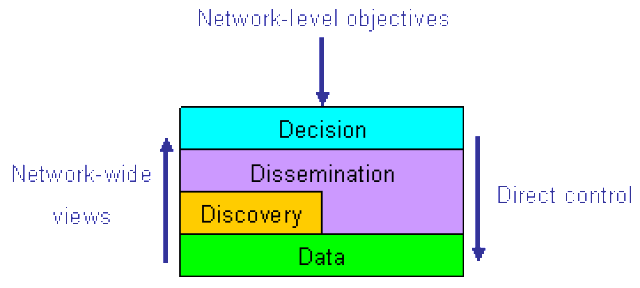
\includegraphics[width=6cm]{4DProject2}
\caption[Capas de la arquitectura 4D]{Capas de la arquitectura 4D}
\label{fig:4DProject}
\end{figure}

En otras palabras el plano de decisión es responsable de crear la configuración de la red, mientras que el plano de diseminación se encarga de recolectar información sobre el estado de la red para el plano de decisión y distribuir la salida del plano de decisión. Mientras tanto el plano de descubrimiento permite a dispositivos descubrir vecinos directamente conectados en la red. Finalmente el plano de datos se encarga de redirigir el tráfico de red.\\ \\

Habiendo introducido a los principales antecedentes de las redes definidas por software, en la siguiente secci\'on se propone abordar el abordaje de dicho concepto.

\section{Software Defined Networking}
\label{section2.2}

Definir el concepto de Software Defined Networking no es una tarea simple, puesto que no se encuentra por completo estandarizado a pesar de la existencia de varias organizaciones trabajando en la temática. En particular se pueden destacar el grupo de trabajo Software-Defined Networking Research Group(SDNRG) del IRTF, quien se encuentra trabajando en la redacción de las definiciones y estándares para este concepto, la Open Networking Foundation(ONF) organización que concentra gran cantidad de material y documentación sobre SDN y se encuentra trabajando en el desarrollo del protocolo OpenFlow el cual se explica mas adelante en este trabajo.\\

Acorde a la Open Networking Foundation, SDN puede resumirse como:

\begin{quote}
\textit{``La separación física del plano de control de la red del plano de datos, y donde el plano de control controla varios dispositivos.''}
\end{quote}

Más en detalle, SDN es una arquitectura de red que desacopla los planos de control y de datos, moviendo el plano de control (inteligencia de la red, construcción y c\'alculo de políticas de red) hacia una entidad denominada Controlador. Esto habilita al control de la red a ser directamente programable y a la infraestructura subyacente ser abstraída por las aplicaciones y servicios de red.\\ 

La ONF presenta a SDN como una arquitectura emergente, dinámica, escalable, rentable y adaptable, haciéndola ideal para aplicaciones de naturaleza dinámica y exigentes de los recursos de red disponibles. En particular destaca las cualidades de presentar una gestión centralizada y de estar basada en estándares abiertos neutrales a los vendedores.\\

\begin{figure}[htbp!] 
\centering    
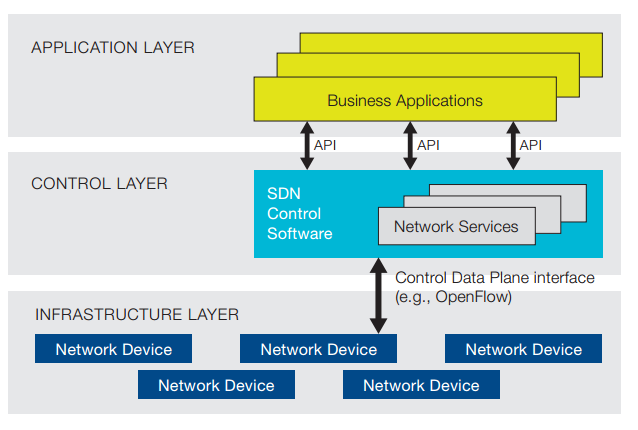
\includegraphics[width=10cm]{SDNArchitecture}
\caption[Arquitectura de SDN - Capas lógicas]{Arquitectura de SDN - Capas lógicas}
\label{fig:SDNArchitecture}
\end{figure}

El enfoque de SDN propone tres capas lógicas(ver imagen ~\ref{fig:SDNArchitecture}): (1) capa de aplicaciones (Application Layer), (2) capa de control (Control Layer) y (3) capa de infraestructura (Infraestructure Layer).\\

La capa de infraestructura se compone por los dispositivos de red tradicionales como switches y routers, en particular compatibles con la arquitectura SDN. La inteligencia de dichos dispositivos a diferencia de switches y routers convencionales es retirada de los mismos para ser trasladada a la capa de control.

Cada dispositivo implementa una API de operaciones bien definida mediante la cual es manipulado por la capa de control. Esta api de operaciones implementa lo que se denomina Interfaz Sur.
\\

En la capa de control se encuentra el software encargado de implementar el plano de control en dicho modelo, usualmente denominado Controlador.

El Controlador implementa una API de operaciones a ser expuestas a las aplicaciones de la capa de Aplicación para la manipulación de dispositivos en la capa de infraestructura. Esta API de operaciones implementa lo que se conoce en el modelo como Interfaz Norte.\\

Por otro lado la capa de aplicaciones contiene implementados en software en forma de aplicaciones toda la inteligencia que originalmente se agregaba en un dispositivo de la capa de infraestructura, por ejemplo la implementaci\'on de protocolos de red.

En dicha capa se pueden implementar desde protocolos de ruteo como OSPF y RIP, backbones sobre MPLS, políticas de seguridad y hasta aplicaciones de ingeniería de tráfico.\\

De esta forma Software Defined Networking centraliza el control de la red en una aplicación de software (Controlador) y transforma algoritmos, procesos de control, políticas de seguridad y toda la inteligencia antiguamente acoplados a los dispositivos de red, en aplicaciones de controlador.\\

\section{Arquitecturas basadas en SDN}
\label{section2.3}

Existen varias arquitecturas o implementaciones en las que de una forma u otra puede encontrarse argumentos para afirmar que siguen el enfoque de SDN. Si bien este trabajo se basa en la utilización de la arquitectura OpenFlow, existen otras arquitecturas basadas en este enfoque como el protocolo ForCES y alternativas m\'as comerciales como OpFlex.

A continuaci\'on se explican los principales conceptos relacionados a la arquitectura OpenFlow.

\subsection{OpenFlow}

Orientado por el enfoque en tres capas de SDN y bajo la misma premisa de desacoplar completamente los planos de datos y control, OpenFlow\cite{mckeown2008openflow} brinda una implementaci\'on estándar para el mecanismo de comunicación entre las capas de control e infraestructura; Interfaz Sur. En otras palabras, provee de un protocolo de comunicación estándar para manipular los distintos dispositivos de la red y así el plano de datos.\\ 

OpenFlow se basa en tres componentes(ver figura ~\ref{fig:OpenFlowArch}): (1) Controlador OpenFlow compatible, (2) Protocolo OpenFlow y (3) Switch OpenFlow compatible.

  
%OpenFlow logra estandarizar la forma mediante la cual cada entrada de la tabla de flujos en un switch, puede ser modificada externamente (Protocolo OpenFlow), brindando un mecanismo transparente y confiable para la manipulación del plano de datos en los switches compatibles con OpenFlow independientemente del vendedor y fabricante del equipo.\\

%Un switch OpenFlow, como se ilustra en la Figura 6, esta compuesto al menos por 3 partes: (1) Una Tabla de Flujos (Flow Table), con una acción asociada a cada flujo en la misma(Flow table entry) para decirle al switch como procesar cada flujo, (2) un Canal Seguro (Secure Channel) que conecta el switch con un proceso de control remoto (Controlador) permitiendo enviar comandos y paquetes entre el controlador y el switch utilizando (3) el protocolo OpenFlow el cual provee una forma abierta y estándar de comunicación entre el controlador y el switch.\\

\begin{figure}[htbp!] 
\centering    
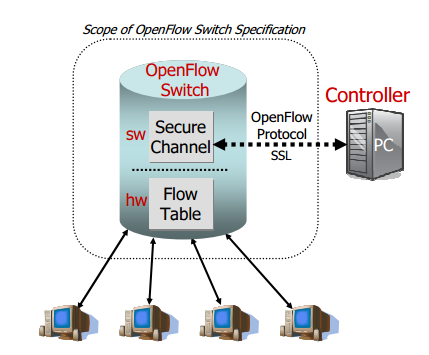
\includegraphics[width=7cm]{OpenFlowArchitecture1}
\caption[Estructura de un switch OpenFlow]{Estructura de un switch OpenFlow. Imagen extraída de \cite{mckeown2008openflow}}
\label{fig:OpenFlowArch}
\end{figure}

Desde la perspectiva de un Controlador OpenFlow, todos los dispositivos de red son equivalentes en sus funcionalidades y se denominan simplemente switches OpenFlow. Un switch OpenFlow se compone de tres componentes principales(ver figura ~\ref{fig:OpenFlowArch}): (1) Tabla de flujos, (2) Canal Seguro (Secure Channel) que conecta el switch con el Controlador habilitando el intercambio de paquetes y comandos entre estos últimos dos utilizando (3) el protocolo OpenFlow.\\
 
Cada switch OpenFlow presenta una o m\'as tablas de flujos. Cada una de las entradas de estas tablas es denominada flujo y determina c\'omo una clase de paquetes deben ser procesados y reenviados.\\

Cada entrada o flujo en esta tabla(ver figura ~\ref{fig:OpenFlowArch2}) se compone de: (1) campos de selección(matching fields), utilizados para identificar a un conjunto de paquetes a ser tratados de una forma en particular, basándose en información relacionada a campos en los cabezales del paquete para esto; (2) contadores para la recolección de información estadística en relación al flujo (n\'umero de paquetes recibidos, cantidad de bytes, duración de un flujo, etc) y (3) un conjunto de instrucciones y acciones que son aplicadas a cada paquete que coincide con el flujo descrito. Estos campos establecen la forma en que un paquete es procesado y reenviado.
 
\begin{figure}[htbp!] 
\centering    
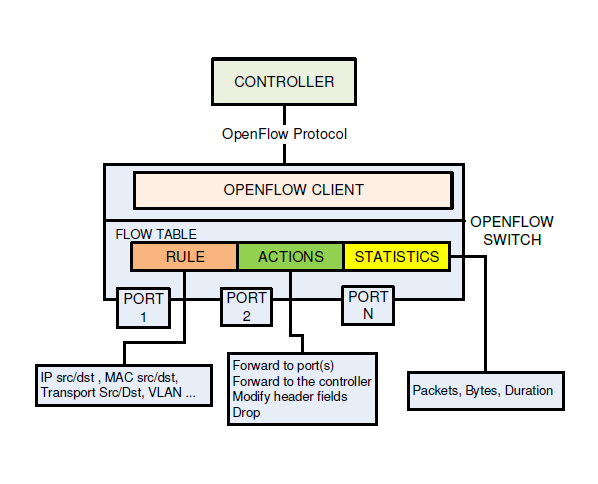
\includegraphics[width=9cm]{OpenFlowArchitecture2}
\caption[Visión esquemática del funcionamiento de un Switch OpenFlow]{Visión esquemática del funcionamiento de un Switch OpenFlow. Imagen extraída de \cite{mckeown2008openflow}}
\label{fig:OpenFlowArch2}
\end{figure}

Cuando un paquete arriba a un switch(ver figura ~\ref{fig:OFPacketProcessing}), se extraen y comparan cabezales del paquete acorde a las reglas definidas en el matching field del flujo, comparando los campos utilizados. En caso que el paquete coincida con las reglas definidas, se aplican el conjunto de instrucciones y acciones asociadas a dicho flujo. En caso que el paquete no coincida con ningún flujo, el accionar a desempeñar dependerá del conjunto de instrucciones y acciones definidas por una entrada especial en la tabla de flujos, denominada Table-miss Flow Entry.\\ 

\begin{figure}[htbp!] 
\centering    
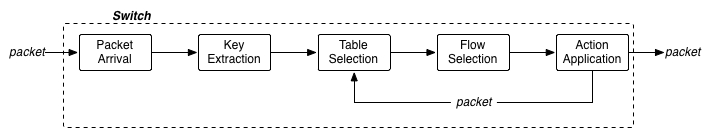
\includegraphics[width=12cm]{OFPacketProcessing}
\caption[Ciclo de vida de un paquete en pipe OpenFlow]{Ciclo de vida de un paquete en el pipe OpenFlow}
\label{fig:OFPacketProcessing}
\end{figure}


La Table-miss Flow Entry esta pensada para contemplar el tr\'afico que no es definido por ningún otro flujo, por ello en esencia es el ultimo flujo a ser considerado(menor prioridad) al momento de procesar un paquete. Generalmente tiene asociada la acción de arrojar el paquete (Drop), procesar el paquete en la siguiente tabla de flujos(GoTo Table) \'o reenviar el paquete al Controlador.\\

Otra caracter\'istica importante de un switch OpenFlow, es la capacidad para procesar paquetes utilizando protocolos tradicionales de red adem\'as del procesamiento normal de OpenFlow. Esta característica a su vez da lugar a la clasificaci\'on en switches OpenFlow puros y switches OpenFlow h\'ibridos. Mientras que los switches OpenFlow puros son aquellos que solamente soportan el protocolo de igual nombre, los switches OpenFlow h\'ibridos son aquellos que adicionalmente permiten procesar paquetes de la misma forma en que lo har\'ia un hardware de red legado.

Aprovechando las capacidades de un switch OpenFlow h\'ibrido, se puede definir por ejemplo la Table-Flow-Entry de forma que se procese todo paquete contemplado por esta entrada como un hardware de red tradicional, aplicando por ejemplo esquemas de reenvío IP. 

\subsection{Reglas OpenFlow}
Cada entrada en la tabla de flujos, distingue un tipo de tr\'afico en particular y la forma en que se procesa(acciones e instrucciones). Es uno de los pilares del protocolo la expresividad disponible para escribir las reglas de cada flujo; es decir, la capacidad de agrupar tipos de tr\'afico acorde a diferentes propiedades en el mismo.\\

\begin{figure}[h] 
\centering    
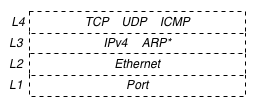
\includegraphics[width=6cm]{ofv1MF}
\caption[OF 1.0 Matching Fields]{OpenFlow v1.0 Matching Fields}
\label{fig:OF10MatchingFields}
\end{figure}

Las reglas OpenFlow se basan en los valores de cabezales asociados a diferentes capas del stack OSI. Estos cabezales a su vez varían con la versi\'on del protocolo, incorporándose m\'as opciones en cada versi\'on del mismo. Por ejemplo en la versi\'on 1.0 del protocolo se tiene un soporte mínimo para cabezales de capas 1 a 4 (ver imagen ~\ref{fig:OF10MatchingFields}).

Por otro lado en la version 1.3.3 del protocolo se cuenta soporte para utilizar cabezales de IPv6, ICMPv6 y MPLS en la definición de los flujos (ver imagen ~\ref{fig:OF13MatchingFields}).
 
\begin{figure}[ht] 
\centering    
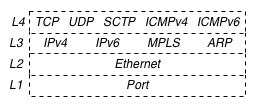
\includegraphics[width=6cm]{ofv13MF}
\caption[OF 1.3.3 Matching Fields]{OF 1.3.3 Matching Fields}
\label{fig:OF13MatchingFields}
\end{figure}

\subsection{Acciones OpenFlow}

Como se menciona anteriormente la acci\'on de un flujo OpenFlow determina la forma en que un paquete es procesado en un switch. Las tres acciones principales que todo switch OpenFlow debe implementar son:

\begin{enumerate}
\item \textbf{[Output:Puerto]:} Reenviar un paquete hacia un puerto determinado (o conjunto de puertos). Esto permite encaminar paquetes a través de la red.

\item \textbf{[Output:Controller]:} Encapsular y reenviar un paquete hacia el Controlador. Utilizando el canal de comunicación con el Controlador y el protocolo OpenFlow, se reenvía el paquete al plano de Control. Esto permite procesar un paquete no identificado en ningún flujo en cualquier momento o en una etapa de configuración de la red. Luego el Controlador decide si descartar el paquete o instalar un nuevo flujo que lo contemple.

\item \textbf{[Drop]:} Descartar un paquete. Puede ser utilizado por razones de seguridad, para prevenir ataques de negación de servicios (DoS), eliminar paquetes sospechosos, disminuir el impacto de paquetes de descubrimiento en redes de difusión(broadcast), o simplemente descartar paquetes no contemplados.
\end{enumerate}

\subsection{Controlador OpenFlow}
Basicamente un controlador SDN brinda implementaciones a las Interfaces Sur y Norte. Un controlador OpenFlow/SDN requiere adem\'as de esto la compatibilidad con el protocolo OpenFlow en la interfaz sur. 

Basándose solamente en estos principios, las implementaciones de controladores OpenFlow pueden ser muy variadas. Desde controladores muy simples como NOX\cite{ControllersNOX} y POX\cite{ControllersPOX} que siguen estrictamente el enfoque de SDN/OpenFlow, hasta controladores m\'as elaborados como OpenDaylight\cite{ControllersOpendaylight} (ver imagen ~\ref{fig:OpenDayLightHydrogen}) que implementan OpenFlow como una característica mas de su implementaci\'on de interfaz Sur.

Sin embargo existen aspectos relacionados a la entidad Controlador dentro del enfoque SDN/OpenFlow que son afines a cualquier implementacion y arquitectura. A continuaci\'on se mencionan los principales:
  
\begin{figure}[ht!] 
\centering    
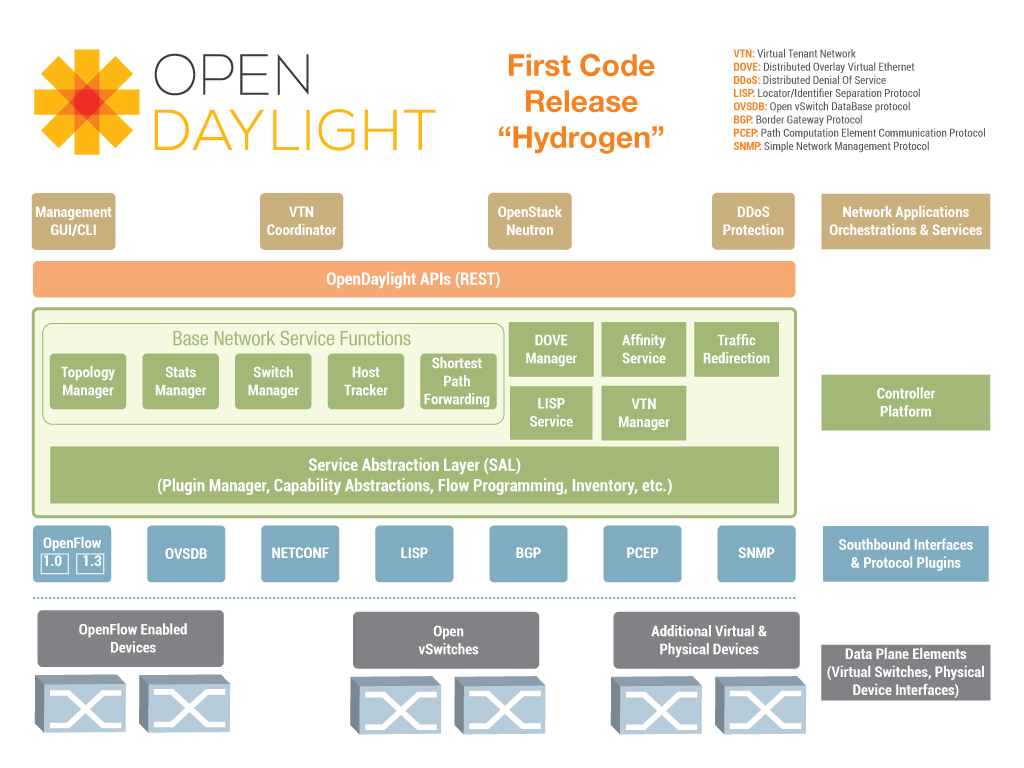
\includegraphics[width=1\textwidth]{opendaylight-hydrogen}
\caption[OF 1.3.3 Matching Fields]{Arquitectura de OpenDaylight Hydrogen}
\label{fig:OpenDayLightHydrogen}
\end{figure}

\subsubsection{Granularidad en el control}
Tradicionalmente, la unidad básica de tráfco en una red es el paquete. Cada paquete contiene información de direccionamiento necesaria para la toma de decisiones dentro del switch a nivel de reenvío. Sin embargo muchas aplicaciones de red envían datos como un flujo de muchos paquetes individuales, mientras que las redes que desean proveer de calidad de servicios(QoS) se benefician utilizando flujos. Por ello resulta beneficioso adoptar un nivel de abstracción superior en el control del plano de datos, distinguiendo tr\'afico por flujos y a través de paquetes individuales.\\
 
Por otro lado uno de los puntos vulnerables del enfoque SDN, es la comunicación entre switch y Controlador. Sobrecargar este canal de comunicación, pensando en redes a gran escala en la cantidad de dispositivos, supone una debilidad importante. Basar la granularidad de control en paquetes individuales, profundiza esta debilidad; mientras que el enfoque basado en flujos atenúa esta debilidad. 

Para fijar ideas, en el caso en que un paquete no es contemplado por un flujo particular y es reenviado al Controlador, puede resolverse instalar un flujo a posteriori para contemplar tal paquete. En el enfoque de flujos, cualquier otro paquete contemplado por el flujo no es m\'as reenviado al Controlador, mientras que en el enfoque de paquetes individuales la regla instalada contempla solamente al paquete inicial.

A su vez se pueden utilizar las mismas prácticas que se utilizan con el control a nivel
de paquetes individuales, como agrupar flujos relacionados al tráfico entre dos hosts, tomando
decisiones sobre los flujos agregados. 

\subsubsection{Centralizado vs Distribuido}
SDN no establece ninguna restricción en cuanto a si el plano de control debe ser tanto lógica como físicamente centralizado o distribuido. De hecho resulta conveniente pensar en enfoques distribuidos cuando se piensa en arquitecturas robustas y escalables. No es el objetivo de este trabajo profundizar en esta área de investigación por lo cual se recomienda para profundizar sobre esta temática \cite{heller2012controller}\cite{levin2012logically}. 

En relacion a OpenFlow, si bien el protocolo no establece mecanismos para la comunicación entre controladores, habilita a un switch a conectarse a múltiples controladores.\\

Algunos proyectos como Onix\cite{koponen2014distributed} e HyperFlow\cite{tootoonchian2010hyperflow} toman la idea de mantener un plano de control lógicamente centralizado, pero físicamente distribuido. Este enfoque tiene como principal beneficio disminuir la sobrecarga en el proceso de búsqueda sobre una tabla de flujos, permitiendo la comunicación con controladores locales.\\

Kandoo\cite{hassas2012kandoo}, proponen utilizar controladores locales para el manejo de aplicaciones y redirigir hacia un Controlador global flujos que requieran de una visión global del estado de la red, bastante similar a lo anterior. Esto tiene como principal beneficio la reducción de la carga sobre el Controlador global, debido al filtrado de solicitudes de flujo que realizan los controladores locales, y a la vez proveen al plano de datos de una rápida respuesta para las solicitudes que pueden ser manejadas por los controladores locales.\\

Concluyendo con este apartado, otro de los enfoques que buscan generar una distribución del plano de control en SDN es el asumido por FlowVisor\cite{sherwood2010carving}. Este enfoque propone la virtualización de una red de switches OpenFlow con múltiples controladores, construyendo lo que denominan Slices de la red. De esta forma brindan a cada controlador una visión local a su slice; mientras que un controlador especial actuá de proxy, manteniendo una visión global de toda la red.

\subsubsection{Políticas reactivas vs proactivas}
Existen dos enfoques para la intervención del controlador en el plano de datos: (1) reactivo y (2) proactivo.

\begin{enumerate}
\item \textbf{Instalación reactiva de políticas:} En este enfoque, para fijar ideas, un switch se configura con la tabla de flujos vac\'ia o al menos una configuración mínima al encenderse. Luego, cada vez que un paquete arriba al switch y no es contemplado por ning\'un flujo, es reenviado al Controlador. Este decide que hacer con el paquete e instala un flujo en el dispositivo para procesar de igual forma paquetes similares.

Este modelo adoptado en particular por Ethane\cite{casado2007ethane}, presenta como principal desventaja la sobrecarga en el canal de comunicación Switch-Controlador. Por ello juega un rol sumamente importante en este esquema la definición de los flujos (flujos m\'as generales disminuyen la sobrecarga con el controlador y flujos muy específicos aumentan esta sobrecarga), tiempo de vida de los flujos en la tabla(flujos con tiempo de vida de un solo paquete aumentan la sobrecarga), la ubicación física del controlador y las características del canal de comunicación. Utilizando una jerarquía de controladores, canales de comunicación de alta velocidad o redundancia de enlaces, se puede mejorar la penalizaci\'on en los tiempos de respuesta por la sobrecarga del canal de comunicación. 

\item \textbf{Instalación proactiva de políticas:} En este enfoque, para fijar ideas, un switch se configurar con la mayor cantidad de flujos posibles, contemplando la mayor cantidad de tr\'afico en la red al momento de encender el switch. Luego, cuando un paquete ingresa al switch, en caso de no ser contemplado por ninguno de los flujos instalados, se reenvía al Controlador para decidir c\'omo actuar. Luego el Controlador puede instalar un flujo para contemplar el caso asociado a este paquete. 

En \cite{yu2011scalable} se analiza el impacto de utilizar un enfoque de políticas proactivas en la performance de una red.  

\end{enumerate} 

%\subsubsection{Escalabilidad}
%[No se si aplique hablar de esto capaz es mucho]

\section{Herramientas SDN/OpenFlow disponibles}

La principal herramienta para el desarrollo de aplicaciones SDN/OpenFlow es el software de control o Controlador. No obstante también existen entornos de emulación compatibles con estas tecnologías y que merecen la pena ser mencionados en este trabajo por su utilidad.

\subsection{Controlador}
Existe un cantidad interesante de propuestas para la implementaci\'on del plano de control. En este trabajo se ha mencionado algunos como OpenDaylight, NOX y POX, pero existen varias alternativas. Pueden encontrarse desde controladores comerciales y académicos, en código abierto y propietario, compatibles solamente con OpenFlow y compatibles con múltiples protocolos incluyendo OpenFlow, etc.\\   

Estas características son utilizadas en este proyecto para la elección de la mejor alternativa de software de control, basándose en las necesidades y restricciones del prototipo. Por ello se cree conveniente incluir el siguiente cuadro comparativo, en el que se presentan las principales características utilizadas en la elecci\'on del controlador m\'as apropiado. Cabe destacar que esta tabla esta basada en una tabla m\'as reducida presentada en \cite{StateOfArt1}. 

\newpage
\begin{table}[!htbp]
\tiny
\begin{tabular}{|l|l|l|p{2cm}|l|p{6cm}|}
\hline   
\textbf{Controlador} & \textbf{Implementación} & \textbf{Opensource} & \textbf{Desarrollador}         & \textbf{OpenFlow} & \textbf{Detalle}                                                                                                                                                                                                                                                                                                          \\
\hline
POX\cite{ControllersPOX}                  & Python                  & Si                  & Nicira                         & 1.0               & Controlador de proposito general implementado en Python, compatible con Linux, Mac OS, y Windows.                                                                                                                                                                                                                         \\
\hline
NOX\cite{ControllersNOX}                  & C++                     & Si                  & Nicira                         & 1.0               & Uno de los primeros controladores ampliamente utilizado. Implementa funcionalidades para descubrimiento de topologías, learning switch, y Network-wide switch.                                                                                                                    \\
\hline
OpenMUL\cite{ControllersOpenMUL}          & C                       & Si                  & Kulcloud                       & 1.4               & Controlador basado en OpenFlow con compatibilidad hacia atrás (OpenFow v1.0, v1.2, etc) con soporte multi-thread basado en lenguaje C, soporte SSL, soporte a múltiples interfaces norte, API REST                                                                                                                        \\
\hline
Maestro\cite{ControllersMaestro}              & Java                    & Si                  & Rice University                & -                 & Maestro es un controlador orientado a la orquestaci\'on de aplicaciones de control de red. Provee de interfaces para el acceso y modificaicon de los dispositivos de la red a estas aplicaciones, as\'i como para coordinar la interacci\'on entre ellas. \\
\hline
Trema\cite{ControllersTrema}                & Ruby/C                  & Si                  & NEC                            & 1.0               & Framework full-stack para el desarrollo de Controladores OpenFlow en Ruby y C, compatible con Ubuntu 13.04 y Fedora 16-19 entre otras distibuciones Linux.                                                                                                                                                                \\
\hline
Beacon\cite{ControllersBeacon}           & Java                    & Si                  & Stanford                       & 1.0?              & Controlador multi-plataforma, rápido y modular basado en Openflow con soporte a programación orientada a eventos y concurrente (threads). Incorpora la plataforma web Jetty y un modulo GUI extensible.                                                                                                                   \\
\hline
Jaxon\cite{ControllersJaxon}                & Java                    & Si                  & Desarrolladores independientes & 1.0?              & Controlador OpenFlow basado en NOX para desarrollo en  Java.                                                                                                                                                                                                                                                              \\
\hline
Helios\cite{ControllersHelios}               & C                       & No                  & NEC                            & -                 & Controlador basado en OpenFlow orientado a lenguaje C, extensible. Interfaz de comunicación Norte en formato Shell.                                                                                                                                                                                                       \\
\hline
Floodlight\cite{ControllersFloodlight}           & Java                    & Si                  & BigSwitch                      & 1.3               & Controlador SDN basado en OpenFlow, soporte para switches virtuales y físicos, maneja redes OpenFlow y redes no OpenFlow así como islas OpenFlow, soporte a OpenStack.                                                                                                                                                     \\
\hline
SNAC\cite{ControllersSNAC}                 & C++                     & No                  & Nicira                         & -                 & Controlador basado en OpenFlow para redes LAN con GUI y un lenguaje definido para declarar reglas. Esta basado en el controlador NOX más un módulo para un lenguaje de modelado formal (FML).                                                                                                                             \\
\hline
Ryu\cite{ControllersRyu}                  & Python                  & Si                  & NTT, OSRG group                & 1.4               & Framework de programación para SDN, provee Controladores basados en OpenFlow, Netconf, Of-config entre otros. Brinda soporte para OpenFlow v1.0 v1.2 v1.3 y v1.4 y extensiones propuestas por le empresa Nicira.                                                                                                                                    \\
\hline
Nodeflow\cite{ControllersNodeFlow}             & Javascript              & Si                  & NTT, OSRG group                &                   & Controlador basado en OpenFlow orientado a programación en Javascript, basado en el framework Node.js.                                                                                                                                                                                                                    \\
\hline
OVS-Controller\cite{ControllersOVS}       & C                       & Si                  & Desarrolladores independientes & -                 & Controlador basado en OpenFlow de referencia con soporte a Open vSwitch y gran parte de otros tipos de switches. Como resultado los switches funcionan como un Switch de capa 2 MAC-learning.                                                                                                                             \\
\hline
FlowVisor\cite{ControllersFlowvisor}            & C                       & Si                  & Stanford/Nicira                & -                 & Controlador de propósitos particulares, que actua como proxy de forma transparente entre una red OpenFLow y múltiples Controladores OpenFlow.                                                                                                                                                                             \\
\hline
RouteFlow\cite{ControllersRouteflow}            & C++                     & Si                  & CPqD                           & 1.3               & Proyecto opensource que provee de servicios de routing virtualizados sobre hardware OpenFlow. Un escenario de uso común puede ser su utilización en conjunto con otro Controlador com Ryu.                                                                                                                                \\
\hline
OpenDaylight\cite{ControllersOpendaylight}         & Java                   & Si                  & Linux Foundation               & 1.3               & Open Daylight es un framework abierto a la comunidad y apoyado por fabricantes, orientado a mejorar y agilizar la adopción de nuevos protocolos y aplicaciones así como e innovación. Este controlador esta desarrollado en java y provee diferentes m\'odulos de conexión para la interfaz Sur, entre los cuales se encuentra el protocolo OpenFlow. Brinda soporte al protocolo OpenFlow hasta versión 1.3 actualmente.\\
\hline   
\end{tabular}
\caption{Controladores disponibles y sus características (Basada en una tabla similar y más reducida en \cite{StateOfArt1})}
\label{table:Controladores}
\end{table}

\subsection{Mininet y Mini Next}
Mininet\cite{Mininet1} es un emulador de red, que habilita a crear hosts, switches, links y controladores, en un entorno virtual. Se encuentra disponible tanto para instalarse nativamente en un entorno Linux, como a través de una m\'aquina virtual configurada con todo el software de desarrollo necesario para iniciarse en el desarrollo de aplicaciones OpenFlow/SDN(Mininet Kit Starter). 

Soporta diferentes versiones del protocolo OpenFlow y es una de las herramientas m\'as utilizadas para la prototipaci\'on y experimentación de aplicaciones desarrolladas en dicha arquitectura; puesto que habilita a investigadores y desarrolladores, aprender, prototipar, probar y debuggear aplicaciones rápidamente utilizando una computadora convencional.\\

Mininext es una extension de Mininet que permite entre otras cosas asignar a cada host su propio sistema de ficheros, permitiendo as\'i modificar la configuraci\'on por defecto de cada nodo virtual e instalar diferentes herramientas en ellos. Esta orientado al despliegue virtual de arquitecturas m\'as complejas que las posibles con Mininet.\\   

En este trabajo Mininet es utilizado para realizar pruebas de experimentaci\'on y benchmark con las alternativas de controladores disponibles, con el objetivo de determinar el controlador OpenFlow a ser utilizado en la arquitectura del prototipo.\\

\section{Aplicaciones de SDN}
SDN presenta un campo de aplicación bastante extenso, y es posible que a medida que el concepto siga evolucionando y asentándose se irán descubriendo nuevos casos de uso y campos de aplicación. A continuación se muestran algunos casos de uso:

\begin{itemize}

\item \textbf{Monitoreo de Red:}
En una arquitectura OpenFlow por ejemplo, cada switch provee de información estadística(similar a SNMP) de cada flujo en tiempo real. De esta forma un Controlador puede recolectar información estadística sobre el tráfico en el plano de datos, lo cual es de gran interés para operadores de red y aplicaciones, con la granularidad exacta que estos requieran. Esta información puede ser agregada de diferentes formas: por dirección IP, por dirección MAC, etiquetas VLAN, por aplicación, etc. De esta forma se logra una gran versatilidad en la entrega de información estadística sobre el tráfico en una red.

\item \textbf{Redes Tap programables:}
Utilizando OpenFlow se pueden implementar redes taps programables y replicar el tráfico para su monitoreo de una forma más eficiente que los métodos tradicionales de SPAN/RSPAN. También pueden filtrarse los datos que son enviados por ejemplo a un sistema de detección de intrusos(IDS), reduciendo la carga de trabajo a los dispositivos de procesamiento de datos utilizados, filtrando previamente los datos que son realmente necesarios y evitando replicar datos innecesarios.\\
Además desde que el control de los dispositivos intermediarios puede realizarse desde un controlador, se facilita enormemente a gestión de los mismos, permitiendo una configuración dinámica en caso de fallas o averías técnicas.

\item \textbf{Balanceo de carga y QoS:}
Contar con una visión global de los dispositivos del plano de datos, habilita al Controlador a implementar diferentes políticas de balanceo de carga en función del estado de la red y permite un uso óptimo de todos los recursos disponibles. A su vez se pueden priorizar diferentes tipos de tráfico, encaminar tráfico dependiendo de un tipo de servicio o contenido y otras técnicas de QoS.

\item \textbf{Herramientas para mitigación de ataques DoS:}
Herramientas para la mitigación de ataques de negación de servicios (DoS) pueden beneficiarse de las estadísticas provistas por un switch OpenFlow por ejemplo para detectar anomalías. Además utilizando la acción de redirección de un flujo al Controlador, se puede analizar y detectar tráfico sospechoso de ataques DoS, permitiendo a posteriori insertar un flujo en el switch de ingreso específico para bloquear el tipo de ataque o tráfico malicioso detectado.

\item \textbf{Inserción de Servicios:}
Con una arquitectura basada en SDN como openFlow, resulta sumamente sencillo la incorporación de servicios al plano de datos de una infraestructura de red dada. Independientemente de la marca del hardware utilizado, sus características y funcionalidades, siempre que sean compatibles con OpenFlow puede incorporarse nuevos servicios como autenticación, cortafuegos, almacenamiento secundario, etc., simplemente programando una nueva aplicación en el Controlador que implemente dichos servicios.

\item \textbf{Experimentación:}
El desarrollo, verificación y puesta en producción de nuevos servicios y protocolos resulta sumamente sencillo puesto que consta simplemente de desplegar una nueva aplicación en un entorno de software (Controlador). Por ello resulta sumamente útil el enfoque de SDN para la academia y la industria en lo que refiere al desarrollo de nuevos protocolos de red, nuevos servicios, mejoras a servicios existentes, entre otros.

\end{itemize}

Por estas razones soluciones basadas en el enfoque SDN con OpenFlow por ejemplo, u otras arquitecturas basadas en SDN resultan de gran utilidad en escenarios como:

\begin{enumerate}
\item Redes empresariales
\item Centros de cómputo(Data Centers)
\item Academia
\end{enumerate}

\section{Casos de éxito de SDN}
OpenFlow en particular se ha hecho con un cierto protagonismo recientemente. Tal es el hecho que se pueden nombrar casos de éxito en la migración de servicios sobre esquemas tradicionales de redes a SDN/OpenFlow.\\

La Open Networking Foundation en particular elabor\'o un articulo\cite{ONFSuccessCase} en donde se recomiendan métodos y se proveen guías para la migración de servicios desde un esquema tradicional a SDN, nombrando en particular tres casos de éxito en este tipo de migraciones, en escenarios reales: (1) Google InterDatacenter WAN, (2) NTT Provider Edge y (3) Stanford Campus Network.

A continuaci\'on se explica en detalle el primer caso de exito, en relaci\'on a los otros dos casos se sugiere continuar la lectura en \cite{ONFSuccessCase}.

\textbf{Google InterDatacenter:}\\

Los servicios de Google orientados a usuarios de Internet como su motor de búsquedas, Google+, GMail, Youtube, Google Maps, entre otros, requieren que una gran cantidad de datos sean movidas desde una región a otra todo el tiempo, haciendo a estas aplicaciones y servicios consumidores intensivos de la WAN. Debido a esto Google concluy\'o que la oferta de dichos servicios no sería escalable con las tecnologías disponibles actualmente, debido a la complejidad en la configuración y manejo de dichas tecnologías las cuales no son lineales con el crecimiento en la demanda de dichos servicios. Como resultado, Google decidió apostar por el enfoque de SDN para el manejo de su WAN. Si el lector est\'a interesado en esta experiencia, puede encontrar una descripción completa en \cite{jain2013b4}.

%\item NTT Provider Edge:

%En el modelo de despliegue tradicional de BGP, los routers  proveedores de servicios de borde(Provider Edge Roputer), mantienen numerosas adyacencias BGP; tantas como routers/caminos BGP para diferentes familias de direcciones, como IPv4, IPv6, VPNv4, VPNv6, etc.\\
 
%Mantener la máquina de estados de BGP, procesar las actualizaciones BGP y configuraciones de políticas, calcular los mejores caminos para cada familia de direcciones, constituyen una gran carga de procesamiento en el hardware del router. Adicionalmente los servicios por definición están sujetos a modificaciones en el tiempo, ya sea para proveer de servicios a nuevos clientes como para actualizar sus políticas. Por otro lado los recursos disponibles como CPU y memoria son limitados, y la naturaleza de los sistemas operativos y hardware de cada equipo es propietaria de la implementación de cada fabricante. Esto limita la aceleración de servicios y la innovación a las políticas de cada vendedor de hardware.\\

%Por ello BGP free edge, define un nuevo paradigma que simplifica el encaminamiento eBGP en los routers PE. En este modelo de despliegue, el router PE se convierte en un nodo de reenvío para manejar el plano de datos, mientras que el plano de control BGP se desacopla a una entidad externa. El plano de control de SDN/Openflow encaja perfectamente en el rol de dicha entidad.\\

%Algunas de las razones por las cuales apostar por BGP free edge:
%\begin{itemize}
%\item Simplificar y abaratar la arquitectura de un router PE-BGP con una política BGP centralizada.
%\item Acelerar el despliegue de nuevos servicios de borde mediante la separación en plano de control y %plano de datos
%\item Mejor control sobre patrones de tráfico
%\item Flexibilidad para calcular mejores caminos configurables
%\item Reducción del efecto ``BGP Wave'', ayudando a la escalabilidad de Internet.
%\end{itemize}

%\item Stanford Campus Network:

%Una parte de la red del campus de la Universidad de Stanford, fue exitosamente migrada para soportar %OpenFlow en el año 2010.
%Inicialmente esta migración fue orientada a usuarios en particular (wireless), luego se agregaron los %usuarios físicamente conectados por cable en el ala 3A del edificio William Gates, y finalmente se %expandió en múltiples islas a través de 2 edificios.

%\end{enumerate}

\section{Red Privada Virtual}
\label{section2.7}

En pocas palabras una Red Privada Virtual \'o VPN por su sigla en ingl\'es, es la extension de una red privada sobre una infraestructura de red p\'ublica como lo es por ejemplo Internet.

Este concepto habilita a un equipo en una determinada subred privada a enviar y recibir información a otro equipo en otra subred separadas f\'isicamente, utilizando una infraestructura de red p\'ublica o compartida para la comunicaci\'on entre ambas subredes, y de la misma forma que si estuviese directamente conectada a la red privada. Adem\'as permite mantener las políticas de seguridad y funcionalidades de la red privada.\\

%Conceptualmente se han propuesto tres arquitecturas b\'asicas de redes VPN: (1) VPN de acceso remoto, (2) VPN punto a punto y (3) VPN sobre LAN.\\

Las implementaciones de redes privadas se caracterizan entre otras cosas por las funcionalidades que son capaces de proveer. En relaci\'on a aspectos de seguridad se buscan principalmente funcionalidades de autenticaci\'on de usuarios, confidencialidad e integridad de los datos. Por otro lado en relaci\'on al procesamiento del tr\'afico dentro de la red p\'ublica, algunas implementaciones de VPN ofrecen funcionalidades de clasificaci\'on de tr\'afico y calidad de servicios (QoS), permitiendo por ejemplo garantizar un ancho de banda m\'inimo para el tr\'afico de una organizaci\'on cuando es transportado a trav\'es de la red p\'ublica de una red privada a otra. 

Algunas implementaciones proveen adem\'as la capacidad de priorizar tipos de tr\'afico como por ejemplo el asociado a una aplicaci\'on en particular, o distribu\'ir la carga entre diferentes caminos, lo que se conoce como balanceo de carga.\\

%Pensando en el contexto de la RAU, alguna de estas funcionalidades como la clasificaci\'on de tr\'afico, priorizaci\'on de tr\'afico por aplicaciones y balanceo de carga se adaptan muy bien a los requerimientos existentes para la nueva versi\'on de la misma(RAU2).\\  

En relaci\'on a la implementaci\'on de redes privadas, a lo largo de los años han surgido diferentes alternativas; diferenciándose por las funcionalidades que implementan y tambi\'en por las capas en el stack OSI en la cual operan. Algunos ejemplos son: 

\begin{itemize}
\item VPN tradicionales
	\begin{itemize}
	\item Frame Relay (Capa 2)	
	\item ATM (Capa 2)
	\end{itemize}
	
\item VPNs basadas en CPE
	\begin{itemize}
	\item L2TP (Capa 2)
	\item IPSec (Capa 2)
	\end{itemize}
	
\item VPNs implementadas por proveedores de servicios
	\begin{itemize}
	\item VPN de capa dos con MPLS (Capa 2)
	\item BGP/MPLS VPNs de capa tres(Capa 3)
	\end{itemize}
\end{itemize}

Otra de las características por la cual es interesante diferenciar a dichas implementaciones, es la capacidad de conectar dos o m\'as puntos de una red privada, lo cual da lugar a redes privadas punto a punto \'o multipunto.

\subsubsection{Redes Privadas Punto a Punto}

Las redes privadas punto a punto son un tipo de implementaci\'on orientada a conectar solamente dos extremos de la red de una organizaci\'on, utilizando lo que se denominan t\'uneles sobre la infraestructura de un proveedor de servicios o Internet. T\'ipicamente se utilizan para conectar un cliente con un servidor en una organizacai\'on, o dos edificios de una misma organizaci\'on de una forma simple. 

\begin{figure}[htbp!] 
\centering    
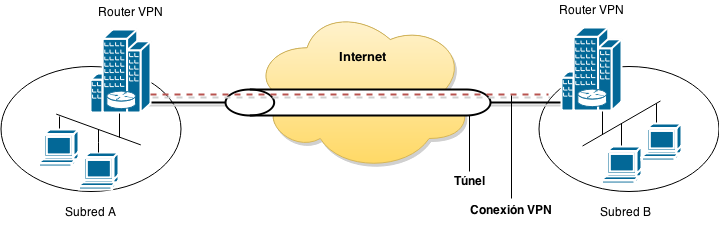
\includegraphics[width=0.7\textwidth]{VPNPuntoaPunto}
\caption[Esquema de una VPN Punto a Punto]{Esquema de una VPN Punto a Punto}
\label{fig:VPNPuntoAPunto}
\end{figure}

En este enfoque el tr\'afico de la subred A al llegar al nodo de borde, es encapsulado y enviado a trav\'es de un túnel sobre la red p\'ublica. Al llegar al otro extremo del túnel el tr\'afico es desencapsulado y entregado al nodo de borde en la subred B, tomando luego el camino correspondiente dentro de esta subred en forma normal. Esto genera la percepci\'on desde ambas subredes que se tiene un “cable” entre ambos nodos de borde, conectando ambas subredes como si fuesen una sola red privada.
 
\subsubsection{Redes Privadas Multipunto}

Las redes privadas multipunto, extienden el enfoque punto a punto con el objetivo de brindar conectividad a una organizaci\'on dispersa geogr\'aficamente en m\'ultiples lugares.

Permiten establecer dominios de difusi\'on compartidos, creando de forma transparente la ilusi\'on de que se tiene una gran LAN compuesta por varias subredes. Sin embargo al ser m\'as completas en funcionalidades y casos de uso soportados, tambi\'en son m\'as complejas de implementar.\\ 

Virtual Private LAN Service(VPLS), es una implementaci\'on de red privada multipunto, bastante difundida y provista de los dos enfoques definidos en los RFC4761\citep{kompella2007virtual} y RFC4762\cite{lasserre2007virtual}. Esta implementaci\'on crea dominios de difusión Ethernet utilizando diferentes tecnologías como IP/MPLS, L2TPv3 y túneles GRE.

\begin{figure}[htbp!] 
\centering    
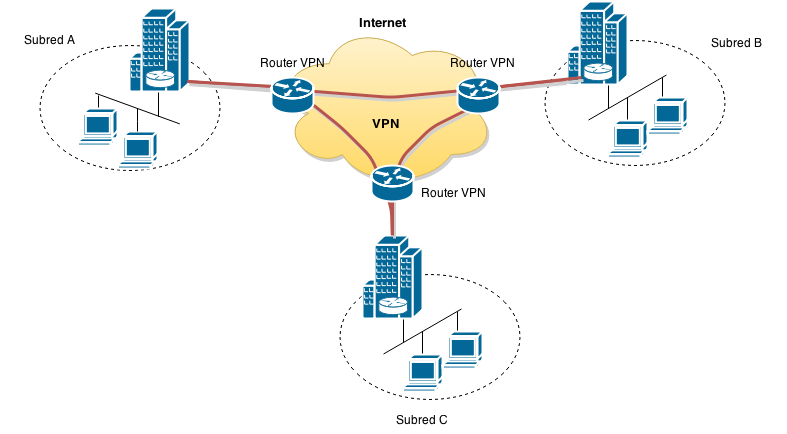
\includegraphics[width=0.7\textwidth]{VPNMultipunto}
\caption[Esquema de una VPN Multipunto]{Esquema de una VPN Multipunto}
\label{fig:VPNMulipunto}
\end{figure}
 
En una red privada multipunto VPLS como la de la figura \ref{fig:OF10MatchingFields}, compuesta por las subredes A, B y C, cuando se origina un paquete en un equipo de la subred A con destino a otro equipo en la subred B sucede lo siguiente: (1) primero el paquete es encaminado al nodo de borde de la subred A (\gloss{Router} VPN), (2) luego se resuelve dinamicamente a que punto de la VPN debe ser enviado el paquete(subred B \'o subred C), para lo cual se utiliza un protocolo de ruteo de borde como BGP, despu\'es (3) el paquete es encapsulado dentro de MPLS y encaminado mediante conmutaci\'on de etiquetas hasta el nodo de borde en la subred B, finalmente (4) el paquete es desencapsulado y entregado a la subred B para su encaminamiento normal hacia el equipo destino.

\subsection{Redes Privadas en Uruguay y proyecciones para la RAU}
En Uruguay ANTEL (el principal proveedor de servicios de telecomunicaciones del país) ofrece servicios de redes privadas basados en tres tecnolog\'ias principalmente: Lan to Lan con conexiones Ethernet punto a punto, VLAN Hub tmbi\'en con conexiones Ethernet y VPN IP/MPLS multipunto con QoS opcionalmente.\\

Dentro de las proyecciones existentes para la RAU2, se encuentran funcionalidades como calidad de servicios, clasificaci\'on de tr\'afico y priorizaci\'on del mismo de acuerdo a pol\'iticas definidas. A su vez se busca conectar m\'ultiples oficinas y organizaciones dispersas geogr\'aficamente en todo el país, manteniendo las pol\'iticas de seguridad de la red privada de cada organizaci\'on. 

De acuerdo a las implementaciones mencionadas anteriormente, la soluci\'on que m\'as se adapta a los requerimientos de la RAU2 es una VPN IP/MPLS multipunto con funcionalidades de QoS, en donde el rol de proveedor de servicios lo asume la propia red académica o la organizaci\'on encargada de su mantenimiento(SeCIU).\\ 

Para complementar la lectura en relaci\'on a la arquitectura de una implementaci\'on de VPN IP/MPLS Multipunto recomendamos continuar con RFC2547\citep{rosen1999bgp} y RFC4364\citep{rosen2006bgp}.

\section{Multiprotocol Label Switching}
\label{section2.8}

Multiprotocol Label Switching(MPLS) o Multiprotocolo de intercambio de etiquetas, es un mecanismo de transporte de datos desarrollado y estandarizado por el IETF, en particular por los RFC 3031\cite{rosen2001multiprotocol}, 3032\citep{rosen2001mpls} y 3814\citep{nadeau2004multiprotocol}.\\

De acuerdo al modelo de capas OSI, MPLS opera entre las capas de Red y Enlace. Fue diseñado para unificar el servicio de transporte de datos basado en circuitos virtuales y basado en conmutación de paquetes.\\

Actualmente cuenta con una gran adopción por parte de vendedores, y poco a poco se ha convertido en el mecanismo por elección para construir plataformas de red empresariales, sustituyendo poco a poco los servicios de Frame Relay y ATM.\\
 
MPLS incluye una gran cantidad de características entre las cuales se distinguen soporte para VPNs, Ingeniería de Tráfico, calidad de servicios (QoS), clases de servicios (CoS), a la vez que es independiente del protocolo de capa de enlace pudiendo operar sobre ATM ó Ethernet por ejemplo.\\

En una red MPLS, cuando un paquete ingresa se le coloca un cabezal mpls. Este cabezal esta compuesto por cuatro campos: Label, Exp, S, TTL. De ellos se destacan el valor de la etiqueta mpls, utilizado para encaminar paquetes a través de la red hacia su nodo destino, y eventualmente realizar clasificación de tr\'afico.

En cada nodo de la red, el cabezal mpls es extraído y analizado para determinar el próximo nodo al que se debe enviar dicho paquete. Luego del procesamiento un nuevo cabezal mpls con otra etiqueta es colocado en el paquete y se reenvía hacia el siguiente nodo en la red.

De esta forma el paquete es encaminado dentro de la red mpls mediante un proceso de extracción y colocación de etiquetas, hasta que el paquete arriba a un nodo de salida de la red, en donde el paquete ya no contiene etiquetas.\\

Por otro lado, un paquete mpls puede presentar más de un cabezal MPLS, uno arriba del otro. Esta superposicion de etiquetas se conoce bajo el nombre de pila o stack mpls. De esta forma se pueden agregar más variables al servicio que simplemente encaminar paquetes en la red, como puede ser distinguir entre diferentes tipos de tráfico.\\

Otro punto a destacar de este protocolo es la configuración del plano de reenvío. El plano de control de las redes mpls se componen de un algoritmo de ruteo y un algoritmo de distribución de etiquetas. Mientras que con el primero se calculan los mejores caminos que un paquete debe tomar para atravesar la red, el segundo se encarga de la asignación y distribución de etiquetas para que cada switch conmute correctamente el paquete hasta su destino.\\

Alguno de los principales términos en la literatura MPLS son:

\begin{itemize}
\item LER(Label Edge Router): Elemento de la red MPLS por la cual ingresa o egresa tráfico hacia o desde la misma.
\item LSR(Label Switching Router): Elemento de la red MPLS que conmuta etiquetas.
\item LSP(Label Switched Path): Nombre genérico que se le asigna a un camino MPLS para tráfico de una determinada FEC, es decir un túnel MPLS establecido entre dos extremos de la red.
\item LDP(Label Distribution Protocol): Protocolo de distribución de etiquetas MPLS entre los equipos de la red.
\item FEC(Forwarding Equivalence Class): Nombre asignado al tráfico que es encaminado bajo una misma etiqueta. En otras palabras, es una clase de equivalencia de tráfico a la cual se le asigna una etiqueta.
 
\end{itemize}
\vspace{1cm}

Hasta ahora, se ha presentado un resumen del trabajo de estudio en el estado del arte en las redes definidas por software y se han introducido los principales conceptos para el correcto entendimiento de este trabajo. Resta entonces presentar las conclusiones obtenidas en el trabajo de estudio del estado del arte del hardware NetFPGA. La siguiente secci\'on esta destinada a esta empresa.

\section{NetFPGA}
\label{section2.9}

NetFPGA\cite{NetFPGA1} es una plataforma de hardware reconfigurable y software opensource, flexible y potente, diseñada para un uso principalmente académico en tareas de investigación y enseñanza.\\

El hardware esta basado en un chip FPGA(Field Programmable Gate Array), el cual se programa con lenguajes de descripci\'on de hardware (HDL) como por ejemplo VeriLog. Cuenta con una amplia variedad de proyectos desarrollados tanto por el equipo de NetFPGA(proyectos de referencia), como por instituciones académicas y comerciales involucradas(proyectos comunitarios) que permiten programar el comportamiento del hardware  de diferentes formas. Se pueden encontrar desde proyectos que programan el hardware con una implementación de referencia de una tarjeta de red (Reference NIC), como un Learning Switch, Simple Router, Router OpenFlow, hasta un generador de tr\'afico entre otros(por mayor informaci\'on ver \citep{NetFPGA2}).\\ 

Surge en el año 2007 como un proyecto de investigación en la Universidad de Stanford, bajo el nombre de NetFPGA-1G, con la consigna de construir una plataforma de desarrollo e investigación basada en un chip FPGA.
 
La plataforma alcanz\'o una versi\'on comercial consistente en una placa PCI con un chip Xilinx Virtex-II proFPGA y cuatro interfaces Ethernet de 1Gigabit, m\'as un repositorio de código fuente descargable y abierto a la comunidad, conteniendo librerías IP y unos pocos ejemplos de diseño.\\

El proyecto prosper\'o vendiendo mas de 2.600 tarjetas en 150 instituciones educativas en 15 países diferentes del mundo hasta el momento en que se discontinuo dicho producto.\\

Tras el éxito de la NetFPGA-1G, en el año 2009 comenzó a trabajarse en la NetFPGA-10G una version m\'as potente que la  anterior basada en un chip Xilinx Virtex5 y cuatro interfaces 10-Gigabit SFP+, que remplazara a la NetFPGA-1G. Tras iniciarse su comercialización en el año 2011 la misma cosech\'o un éxito similar a su antecesora llegando a vender mas de 470 unidades al año 2014, y contando con una plataforma de al menos 15 proyectos desarrollados específicamente para esta plataforma.\\

A la fecha, NetFPGA cuenta con cuatro versiones de plataformas comerciales, la NetFPGA-1G(discontinuada), NetFPGA-10G, NetFPGA CML y NetFPGA-SUME. A su vez la plataforma se ha popularizado entre investigadores y desarrolladores como plataforma ideal para la experimentación e innovación, contando a la fecha con mas de 226 artículos académicos\cite{NetFPGA4} en diversas áreas, utilizando como plataforma de trabajo NetFPGA.\\

En resumen NetFPGA es una plataforma robusta que propicia a investigadores, docentes y estudiantes en el área de redes de computadoras a la construcción de prototipos sobre sistemas de redes de alta velocidad y acelerados por hardware, en poco tiempo y con un costo inferior a otras alternativas de prototipaci\'on.\\

En este trabajo, se utiliza la plataforma NetFPGA-10G para la prototipaci\'on de un dispositivo compatible con OpenFlow, a partir del cual a su vez implementar una red prototipo basada en el enfoque OpenFlow/SDN. 

